\section{A-Stable Backwards Difference}
In the BDF methods, the time derivative is approximated using one-sided finite differences.  The BDF2 method is A-stable, whereas BDF3 is not.  Consider a multi-step method in which the time derivative is approximated by the average of the BDF2 and BDF3 time-derivative approximations:

\begin{equation*}
    \frac{du}{dt} = f \rightarrow \frac{1}{2}\frac{du}{dt}|_{\text{BDF2}} + \frac{1}{2}\frac{du}{dt}|_{\text{BDF3}} = f
\end{equation*}

\begin{enumerate}[label=\alph*., start = 1]
    \item Determine the coefficients $\alpha_k$ and $\beta_k$ that define this method.  What is its order of accuracy?
    
    \vspace{-0.35in}
    \begin{align*}
        \shortintertext{\textbf{\underline{BDF2:}}\newline The expression for the derivative can be expressed as,}
        u_t & = \frac{\frac{3}{2}u^{n+1} - 2u^n + \frac{1}{2}u^{n-1}}{\Delta t} = f^{n+1}\\
        \shortintertext{\textbf{\underline{BDF3:}}\newline The expression for the derivative can be expressed as,}
        u_t & = \frac{\frac{11}{6}u^{n+1} - 3u^n + \frac{3}{2}u^{n-1} - \frac{1}{3}u^{n-2}}{\Delta t} = f^{n+1}\\
        \shortintertext{Averaging BDF2 and BDF3 together will give the time-derivative approximation,}
        \Delta tf^{n+1} & = \frac{1}{2}\underbrace{\left(\frac{3}{2}u^{n+1} - 2u^n + \frac{1}{2}u^{n-1}\right)}_{\text{BDF2}} + \frac{1}{2}\underbrace{\left(\frac{11}{6}u^{n+1} - 3u^n + \frac{3}{2}u^{n-1} - \frac{1}{3}u^{n-2}\right)}_{\text{BDF3}}\\
        \shortintertext{Combining like terms results in,}
    \end{align*}

    \vspace{-0.65in}
    \begin{gather*}
        \frac{5}{3}u^{n+1} - \frac{5}{2}u^n + u^{n-1} - \frac{1}{6}u^{n-2} = \Delta t f^{n+1}\\
        \shortintertext{This results in the coefficients $\alpha$ and $\beta$ to be,}
        \boxed{\alpha_1 = \frac{5}{3},\quad \alpha_0 = -\frac{5}{2},\quad \alpha_{-1} = 1,\quad \alpha_{-2}=-\frac{1}{6},\quad \beta_1 = 1}
    \end{gather*}

    \vspace{-0.25in}
    \begin{align*}
        \shortintertext{\textbf{\underline{Order of Accuracy}}\newline Firstly, is to start with the Taylor-Series expansion expression,}
        u^{n+k} & = u^n + (k\Delta t)u_t^n + \frac{1}{2}(k\Delta t)^2u_{tt}^n + \frac{1}{6}(k\Delta t)^3u_{ttt}^n + \frac{1}{24}(k\Delta t)^4u_{t^{(4)}}^n + \ldots \mathcal{O}(\Delta t^5)\\
        f^{n+k} = u_t^{n+k} & = u_t^n + (k\Delta t)u_{tt}^n + \frac{1}{2}(k\Delta t)^2u_{ttt}^n + \frac{1}{6}(k\Delta t)^3u_{t^{(4)}} + \frac{1}{24}(k\Delta t)^4u_{t^{(5)}}^n + \ldots \mathcal{O}(\Delta t^5)
    \end{align*}
\end{enumerate}

\pagebreak
\pagestyle{fancy}
\restoregeometry

\begin{adjustwidth}{2.5em}{0pt}
    \textbf{\underline{Conducting Taylor-Expansions:}}
    \begin{align*}
        u^{n+1} & = u^n + \Delta t u_t^n + \frac{1}{2}\Delta t^2u_{tt}^n + \frac{1}{6}\Delta t^3u_{ttt}^n + \frac{1}{24}\Delta t^4u_{t^{(4)}}^n + \ldots \mathcal{O}(\Delta t^5)\\
        u^n & = u^n\\
        u^{n-1} & = u^n - \Delta tu_t^n + \frac{1}{2}\Delta t^2u_{tt}^n - \frac{1}{6}\Delta t^3u_{ttt}^n + \frac{1}{24}\Delta t^4u_{t^{(4)}}^n + \ldots \mathcal{O}(\Delta t^5)\\
        u^{n-2} & = u^n -2\Delta tu_t^n +2\Delta t^2u_{tt}^n - \frac{4}{3}\Delta t^3u_{ttt}^n + \frac{2}{3}\Delta t^4u_{t^{(4)}}^n + \ldots \mathcal{O}(\Delta t^5)\\
        f^{n+1} & = u_t^n + \Delta tu_{tt}^n + \frac{1}{2}\Delta t^2u_{ttt}^n + \frac{1}{6}\Delta t^3u_{t^{(4)}}^n + \frac{1}{24}\Delta t^4u_{t^{(5)}}^n + \mathcal{O}(\Delta t^5)\\
        \shortintertext{Then for the order of accuracy the error gives,}
        \epsilon^{n+1} & = \frac{5}{3}u^{n+1} - \frac{5}{2}u^n + u^{n-1} - \frac{1}{6}u^{n-2} - \Delta tf^{n+1}\\
        & = \frac{5}{3}\left(u^n + \Delta t u_t^n + \frac{1}{2}\Delta t^2u_{tt}^n + \frac{1}{6}\Delta t^3u_{ttt}^n + \frac{1}{24}\Delta t^4u_{t^{(4)}}^n \right) + \ldots \\
        & -\frac{5}{2}u^n + \ldots \\
        & + \left(u^n - \Delta tu_t^n + \frac{1}{2}\Delta t^2u_{tt}^n - \frac{1}{6}\Delta t^3u_{ttt}^n + \frac{1}{24}\Delta t^4u_{t^{(4)}}^n\right) + \ldots \\
        & -\frac{1}{6}\left(u^n -2\Delta tu_t^n +2\Delta t^2u_{tt}^n - \frac{4}{3}\Delta t^3u_{ttt}^n + \frac{2}{3}\Delta t^4u_{t^{(4)}}^n\right) + \ldots \\
        & -\Delta t \left(u_t^n + \Delta tu_{tt}^n + \frac{1}{2}\Delta t^2u_{ttt}^n + \frac{1}{6}\Delta t^3u_{t^{(4)}}^n + \frac{1}{24}\Delta t^4u_{t^{(5)}}^n \right)\\
        \shortintertext{Then using Matlab to simplify gives that the error is,}
        \epsilon^{n+1} & = -\frac{1}{6}\Delta t^3u_{ttt} - \frac{1}{6}\Delta t^4u_{t^{(4)}} + \frac{1}{40}\Delta t^5u_{t^{(5)}}
        \shortintertext{Then from the leading term this gives that the convergence is,}
        |\epsilon^{n+1}| & = \mathcal{O}(\Delta t^{p+1}) = \mathcal{O}(\Delta t^3)\\
        \shortintertext{This gives that the order of accuracy is,}
    \end{align*}

    \vspace{-0.5in}
    \begin{equation*}
        \boxed{p = 2}
    \end{equation*}

    \begin{fminipage}{0.9\linewidth}
        \textbf{Since $\bf p = 2$, the order of accuracy for this scheme is second-order accurate. }
    \end{fminipage}

\end{adjustwidth}

\pagebreak
\begin{enumerate}[label=\alph*., start = 2]
    \item Perform an eigenvalue-stability analysis and \textit{prove} (analytically) that this method is A-stable. \newline Plot its stability boundary in the $\lambda\Delta t$ complex number plane, and overlay BDF2 and BDF3.

    \vspace{-0.35in}
    \begin{align*}
        \shortintertext{Starting with the expression for this averaged time-derivative,}
        \Delta t f^{n+1} & = \frac{5}{3}u^{n+1} - \frac{5}{2}u^n + u^{n-1} - \frac{1}{6}u^{n-2}\\
        \shortintertext{Then from here substituting in $g^{n+k}u_0$ for $u^{n+k}$ and $\lambda g^{n+k}u_0$ for $f^{n+k}$,}
        \lambda\Delta t  g^{n+1}u_0  & = \frac{5}{3}g^{n+1}u_0 - \frac{5}{2}g^{n}u_0 + g^{n-1}u_0 - \frac{1}{6}g^{n-2}u_0\\
        \shortintertext{Then taking this expression and dividing by $g^nu_0$ results in,}
        \lambda\Delta t  g  & = \frac{5}{3}g - \frac{5}{2} + g^{-1} - \frac{1}{6}g^{-2}\\
        \shortintertext{Isolating the $\lambda\Delta t$ term then results in,}
        \lambda\Delta t & = \frac{5}{3} - \frac{5}{2}g^{-1} + g^{-2} - \frac{1}{6}g^{-3}\\
        \shortintertext{Further simplifications without loss of generality gives,}
        \lambda\Delta t & = \frac{5}{3} + \frac{1}{6g^3}\left(-15g^2 + 6g-1\right)\\
        \shortintertext{Then by definition, this scheme must be stable if the un-stable region (the regions \textit{inside} the marked plots do not extend into the left-hand plan).  In this limiting case, this can be re-written as the limit as $\lambda\Delta t\rightarrow 0^{-}$ and solve for the $\theta$ value at which this occurs,}
        \lim_{\lambda\Delta t\rightarrow 0} & = 0 = \frac{5}{3} + \frac{1}{6g^3}\left(-15g^2 + 6g-1\right)\\
        \shortintertext{Taking this further, isolating and solving for $g$ gives}
        \lim_{\lambda\Delta t\rightarrow 0} & = -10g^3 = -15g^2 + 6g-1\\
        \shortintertext{Pulling all $g$ terms to one side results in,}
        0 & = 10g^3 -15g^2 + 6g-1\\
        \shortintertext{Conducting simple factorization gives,}
        0 & = \left(g - 1\right)\left(10g^2 - 5g + 1\right)\\
        \shortintertext{Using quadratic formula this gives that $g$ is equivalent to,}
        g & = 1, \frac{5\pm i\sqrt{15}}{20}\\
        \shortintertext{Solving for the values at which these occurs gives,}
        g & = \frac{5\pm i\sqrt{15}}{20} = \exp[i\theta] = \cos{\theta} + i\sin{\theta}\\
        \theta & = 1.1513i \pm 0.6591\\
        \shortintertext{Again for $g=1$,}
        g & = 1 = \exp[i\theta] = \cos{\theta} + i\sin{\theta}\\
        \theta & = 0,\quad \textbf{Physical answer}
    \end{align*}

    \vspace{-0.25in}
    \begin{fminipage}{0.9\linewidth}
        \textbf{As shown above, there are three approximated answers in which this averaged time-derivative scheme will cross into the unstable region. However, two of these three are not physical answers as $\bf \theta \in [0, 2\pi]\ |\ \theta \in \mathbb{R}\ \therefore$ the limiting case occurs at $\bf \theta = 0$ where $g=1$ resulting in $\bf \lambda\Delta t = \frac{5}{3} - \frac{5}{3} = 0$ -- resulting in an \underline{A-stable scheme.}}
    \end{fminipage}
    
    \pagebreak

    Plotting these eigenvalue stability regions can show and confirm that $\theta = 0$ is the limiting case and for the averaged time-derivative that it is indeed A-stable as the unstable region never crosses into the left-hand plane like in BDF3 scheme. Plotting the un-stable regions gives Figure \ref{fig:q1_eigs} shown below,

    \begin{figure}[h]
        \centering
        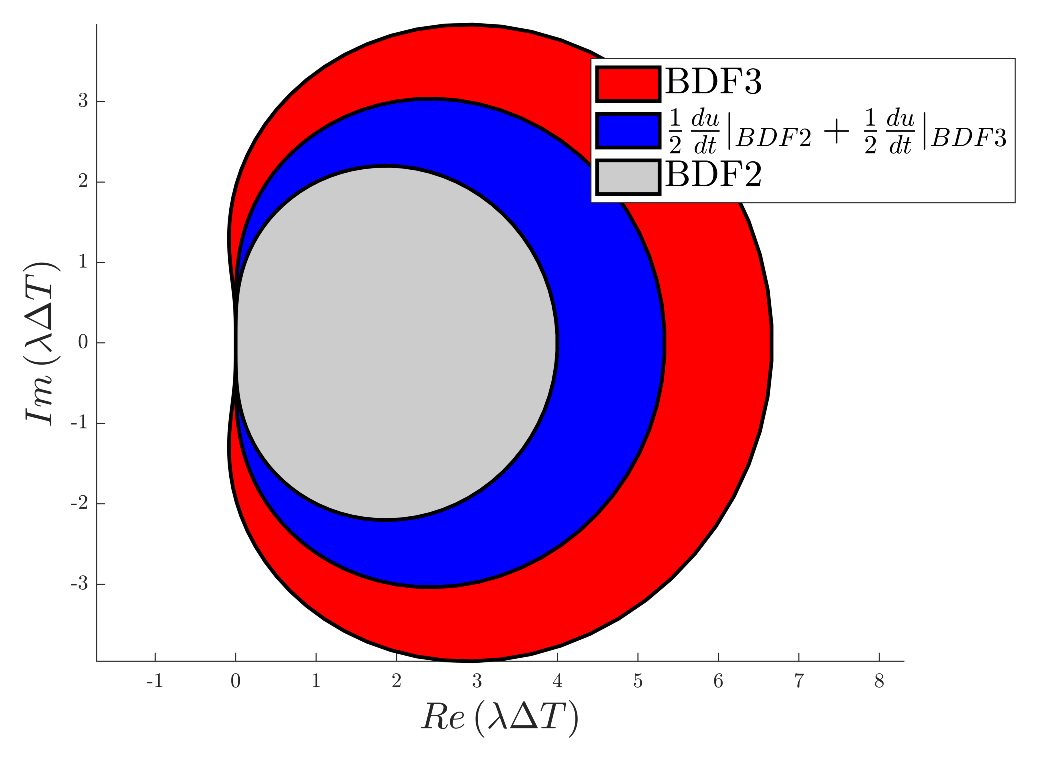
\includegraphics[width = 0.9\linewidth]{q1/eigs.eps}
        \caption{Eigenvalue stability region for BDF2, BDF3, and the averaged time-derivative approximation.}
        \label{fig:q1_eigs}
    \end{figure}

    \begin{fminipage}{0.9\linewidth}
        \textbf{Shown above in Figure \ref{fig:q1_eigs} are the un-stable regions for BDF2, BDF3, and the averaged time-derivative of the two. Outside of these regions the schemes remain stable where the left-hand plane where $\bf Re(\lambda \Delta T) < 0$ is the A-stable region of the schemes.}
    \end{fminipage}
\end{enumerate}

\pagebreak
\begin{enumerate}[label=\alph*., start = 3]
    \item Calculate the temporal truncation error of this method, $\tau= \text{LHS} - \text{RHS}$ of the multistep formula, and show that the leading term is half the magnitude of that of BDF2.    
    

    \vspace{-0.35in}
    \begin{align*}
        \shortintertext{From part a. of this question, I found that the local error was,}
        \epsilon^{n+1} & = -\frac{1}{6}\Delta t^3u_{ttt} - \frac{1}{6}\Delta t^4u_{t^{(4)}} + \frac{1}{40}\Delta t^5u_{t^{(5)}}\\
        \shortintertext{Thus, the truncation error is}
        \epsilon^{n+1} & = \underbrace{-\frac{1}{6}\Delta t^3u_{ttt} - \frac{1}{6}\Delta t^4u_{t^{(4)}} + \frac{1}{40}\Delta t^5u_{t^{(5)}} + \ldots \mathcal{O}(\Delta t^6)}_{\text{truncation error: $\mathcal{O}(\Delta t^3)$}}
        \shortintertext{However, proving that the leading term is half the magnitude of that of BDF2, I will use the LHS and RHS definitions from BDF2 and use the Taylor-Series expansions from part a. and simplify as,}
        \text{LHS} & = \frac{3}{2}u^{n+1} - 2u^n + \frac{1}{2}u^{n-1}\\
            & = \frac{3}{2}\left(u^n + \Delta tu_t^n + \frac{1}{2}\Delta t^2u_{tt}^n + \frac{1}{6}\Delta t^3u_{ttt}^n + \frac{1}{24}\Delta t^4u_{t^{(4)}}^n + \frac{1}{120}\Delta t^5u_{t^{(5)}}^n\right) + \ldots \\
            & - 2u^n + \ldots \\
            & + \frac{1}{2}\left(u^n - \Delta tu_t^n + \frac{1}{2}\Delta t^2u_{tt}^n - \frac{1}{6}\Delta t^3u_{ttt}^n + \frac{1}{24}\Delta t^4u_{t^{(4)}}^n - \frac{1}{120}\Delta t^5u_{t^{(5)}}^n\right)\\
            & = \Delta tu_t^n + \Delta t^2u_{tt}^n + \frac{1}{6}\Delta t^3 u_{ttt}^n + \frac{1}{12}\Delta t^4 u_{t^{(4)}}^n + \frac{1}{120}\Delta t^5u_{t^{(5)}}^n\\
        \text{RHS} & = \Delta t f^{n+1}\\
            & = \Delta t\left(u_t^n + \Delta tu_{tt}^n + \Delta t^2 u_{ttt}^n + \Delta t^3u_{t^{(4)}}^n + \Delta t^4u_{t^{(5)}}^n\right)\\
        \shortintertext{Taking the difference between the two gives,}
        \text{LHS} - \text{RHS} & = \left(\frac{1}{6} - \frac{1}{2}\right)\Delta t^3u_{ttt}^n + \left(\frac{1}{12} - \frac{1}{6}\right)\Delta t^4u_{t^{(4)}}^n + \left(\frac{1}{120} - \frac{1}{24}\right)\Delta t^5u_{t^{(5)}}^n\\
        \tau & = \text{LHS} - \text{RHS} = -\frac{1}{3}\Delta t^3u_{ttt}^n - \frac{1}{12}u_{t^{(4)}}^n - \frac{1}{30}\Delta t^5u_{t^{(5)}}^n\\
        \shortintertext{Then re-writing both truncation errors gives,}
        \tau_{BDF2} & = -\frac{1}{3}\Delta t^3u_{ttt}^n - \frac{1}{12}u_{t^{(4)}}^n - \frac{1}{30}\Delta t^5u_{t^{(5)}}^n\\
        \tau_{\text{Avg}} & = -\frac{1}{6}\Delta t^3u_{ttt} - \frac{1}{6}\Delta t^4u_{t^{(4)}} + \frac{1}{40}\Delta t^5u_{t^{(5)}}
    \end{align*}

    \begin{fminipage}{0.9\linewidth}
        \textbf{By inspection of the truncation errors above, we see that the leading term for the averaged time-derivative is indeed \underline{half} that of the BDF2 scheme.}
    \end{fminipage}

\end{enumerate}
